
\documentclass[%
 %reprint,
%superscriptaddress,
%groupedaddress,
%unsortedaddress,
%runinaddress,
%frontmatterverbose, 
preprint,
%showpacs,preprintnumbers,
%nofootinbib,
%nobibnotes,
%bibnotes,
 amsmath,amssymb,
 aps,
%pra,
%prb,
%rmp,
%prstab,
%prstper,
%floatfix,
]{revtex4-1}

\usepackage{listings}
\usepackage{asymptote}
\usepackage{graphicx}% Include figure files
\usepackage{dcolumn}% Align table columns on decimal point
\usepackage{bm}% bold math
%\usepackage{hyperref}% add hypertext capabilities
%\usepackage[mathlines]{lineno}% Enable numbering of text and display math
%\linenumbers\relax % Commence numbering lines

%\usepackage[showframe,%Uncomment any one of the following lines to test 
%%scale=0.7, marginratio={1:1, 2:3}, ignoreall,% default settings
%%text={7in,10in},centering,
%%margin=1.5in,
%%total={6.5in,8.75in}, top=1.2in, left=0.9in, includefoot,
%%height=10in,a5paper,hmargin={3cm,0.8in},
%]{geometry}
\usepackage[margin=25mm]{geometry}
\usepackage{changepage}
\usepackage{mathcomp}
\usepackage[english]{babel}
\usepackage{siunitx}
\usepackage{tikz}
\DeclareSIUnit\minute{min}
\usepackage{amsmath,mathrsfs,amsfonts,amssymb,amsthm } %permette di mettere formule una sotto l'altra,
%dovrebbe scrivere lettere corsive eleganti con "\mathscr{--},"
% permette di definire insiemi numerici con \mathbb{""},
\usepackage[utf8]{inputenc} %accenti
\theoremstyle{plain} 
\theoremstyle{definition}
\newtheorem{defn}{Def}[section]
\theoremstyle{plain}
\newtheorem{thm}{Theorem}[section] 
\newcommand{\R}{\mathbb{R}}
\newcommand{\N}{\mathbb{N}}
\newcommand{\off}{\text{off}}
\newcommand{\mat}{\text{Mat}}
\newcommand{\B}{\mathbf{B}}
\newcommand{\A}{\mathbf{A}}
%\newcommand{\S}{\mathbf{S}}
\newcommand{\open}{\left}
\newcommand{\close}{\right}
\newcommand{\void}{\varnothing}
\newcommand{\xslash}{\setminus}

%\newcommand{\fnorm}{\lVert #1 \rVert_F}

\usepackage[T1]{fontenc}
\usepackage{subfig}
\usepackage{caption}
\usepackage{subfig}
\usepackage{booktabs}
\usepackage{float}
\usepackage{mathdots}
\usepackage{mathrsfs}
\usepackage{braket}
\usepackage{hyperref}
\usepackage{float}
\usepackage{gensymb}

\usepackage{pgfplots}
\usepackage{circuitikz}
\usepackage{hyperref}
\usepackage{tkz-tab}
\usepackage{caption}
\usetikzlibrary{backgrounds,automata}
\pgfplotsset{/pgf/number format/use comma,compat=newest}
\usetikzlibrary{graphs,shapes,positioning,shadows}

\usepackage{colortbl}
\newcommand{\blue}[1]{\textcolor{blue}{#1}}
\newcommand{\red}[1]{\textcolor{red}{#1}}
\newcommand{\green}[1]{\textcolor{green}{#1}}
\newcommand{\magenta}[1]{\textcolor{magenta}{#1}}
\newcommand{\cyan}[1]{\textcolor{cyan}{#1}}
\newcommand{\yellow}[1]{\textcolor{yellow}{#1}}
\newcommand{\grey}[1]{\textcolor{grey}{#1}}
\newcommand{\abs}[1]{\lvert#1\rvert}

\begin{document}


\title{FYS 3150 - Project 3}% Force line breaks with \\
%\thanks{A footnote to the article title}%


\author{Lorenzo Speri}
\affiliation{University of Oslo, Department of Physics}
%
% Authors' institution and/or address\\
% This line break forced with \textbackslash\textbackslash
%}%

%\collaboration{CLEO Collaboration}%\noaffiliation

\date{\today}% It is always \today, today,
             %  but any date may be explicitly specified
\maketitle

\begin{center}
\section{Abstract}

\end{center}

%\begin{description}
%\item[Usage]
%Secondary publications and information retrieval purposes.
%\item[PACS numbers]
%May be entered using the \verb+\pacs{#1}+ command.
%\item[Structure]
%You may use the \texttt{description} environment to structure your abstract;
%use the optional argument of the \verb+\item+ command to give the category of each item. 
%\end{description}

\begin{itemize}
\item URL to GitHub folder of the code: \url{}
\end{itemize}


%\pacs{Valid PACS appear here}% PACS, the Physics and Astronomy
                             % Classification Scheme.
%\keywords{Suggested keywords}%Use showkeys class option if keyword
                              %display desired


%\tableofcontents
\section{Introduction}
%You don’t need to answer all questions in a chronological order. When you write the introduction you could focus on the following aspects
%Motivate the reader, the first part of the introduction gives always a motivation and tries to give the overarching ideas
%What I have done
%The structure of the report, how it is organized etc


\section{Methods and algorithms}
%Describe the methods and algorithms
%You need to explain how you implemented the methods and also say something about the structure of your algorithm and present some parts of your code
%You should plug in some calculations to demonstrate your code, such as selected runs used to validate and verify your results. The latter is extremely important!! A reader needs to understand that your code reproduces selected benchmarks and reproduces previous results, either numerical and/or well-known closed form expressions.

\begin{table}[h!]
\centering
\setlength{\tabcolsep}{12pt}
\caption{}
\label{time}
\begin{tabular}{ccc}
\toprule
$L$ &  Parallelized code & Normal code \\
\midrule
  40	    &   2.18656 & 7.33698 \\
  60	     &  4.75809 & 17.0014 \\
  80	     &  8.43173 & 29.8397 \\
  100	 &  14.1064 & 46.9271 \\
\bottomrule
 & time in seconds & time in seconds
\end{tabular}

\end{table}

%\begin{equation}
%A(a \to b) = 
%\begin{cases}
%\exp(- \beta(E_b-E_a)) \hspace{0.5cm} if \quad E_b-%E_a>0 \\
%1 \hspace{0.5cm} else
%\end{cases}
%\end{equation}
%\setlength{\unitlength}{2pt}
%\begin{picture}(70,40)(0,-5)
%\newsavebox{\verticalfour} 
%\savebox{\verticalfour}(0,0)[bl]{
%	\multiput(0,0)(0,10){4}{\circle{2}}     % spins
%	\multiput(0,5)(0,10){4}{\line(0,-1){3}} % lines down
%	\multiput(0,-5)(0,10){4}{\line(0,1){3}} %   lines up
%	\multiput(2,0)(0,10){4}{\line(1,0){6}}  % lines right
%}
%\multiput(0,0)(10,0){6}{\usebox{\verticalfour}}
%\end{picture}
%\pagebreak


\section{Results}
%Present your results
%Give a critical discussion of your work and place it in the correct context.
%Relate your work to other calculations/studies
%An eventual reader should be able to reproduce your calculations if she/he wants to do so. All input variables should be properly explained.
%Make sure that figures and tables should contain enough information in their captions, axis labels etc so that an eventual reader can gain a first impression of your work by studying figures and tables only.


%\begin{figure}[h!]
%\centering
%     \subfloat[]{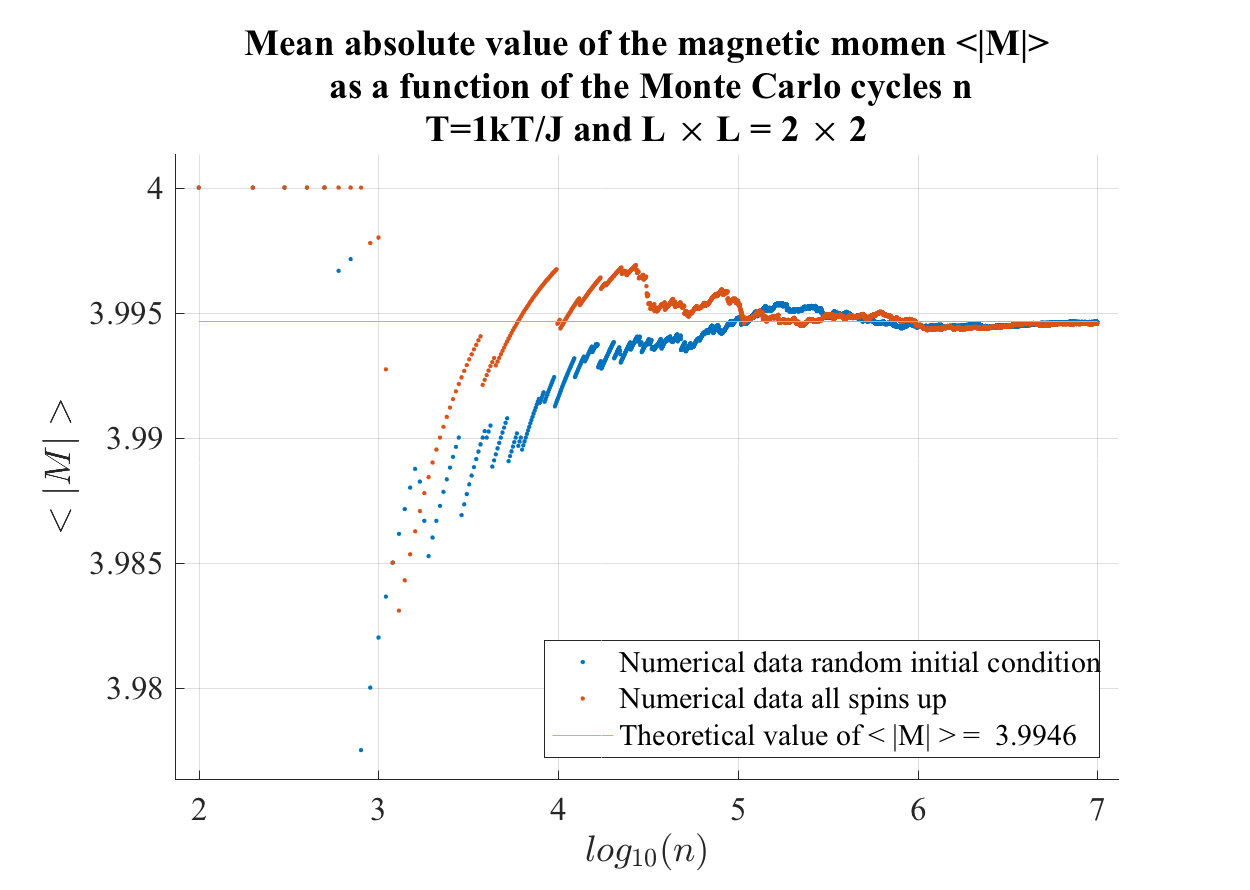
\includegraphics[width=.5\linewidth]{absm2x2.eps}\label{absm2x2}}
%     \subfloat[]{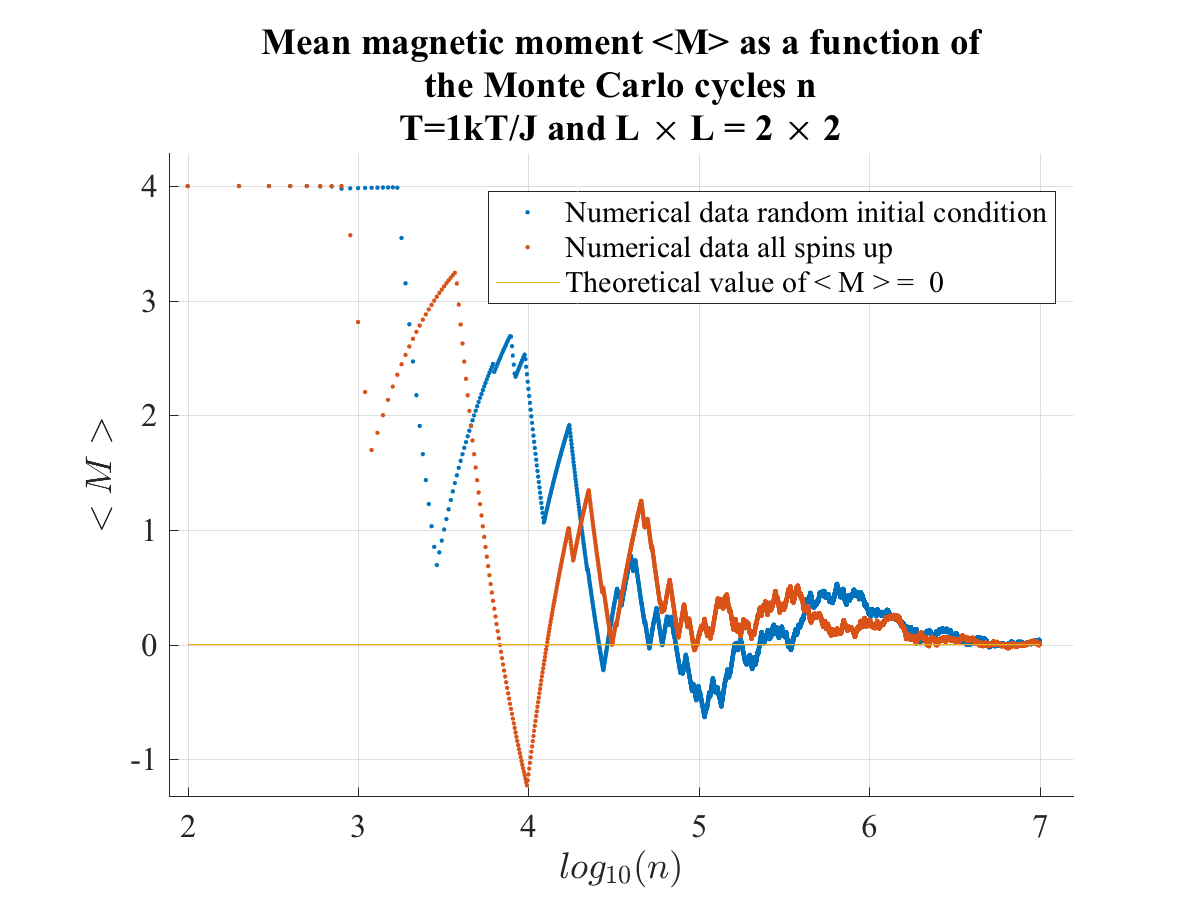
\includegraphics[width=.5\linewidth]{m2x2.eps}\label{m2x2.eps}}
%\caption{In Figure (a) and (b) are shown respectively mean absulute value of magnetization and the mean magnetization as a function of Monte Carlo cycles $n$ for a temperature $T=1 kT/J$ and lattice dimension $L=2$. We can notice that the mean magnetization takes more Monte Carlo cycles before reching a steady state.}
%\end{figure}
 
%\begin{figure}[H]
%\centering
%     \subfloat[]{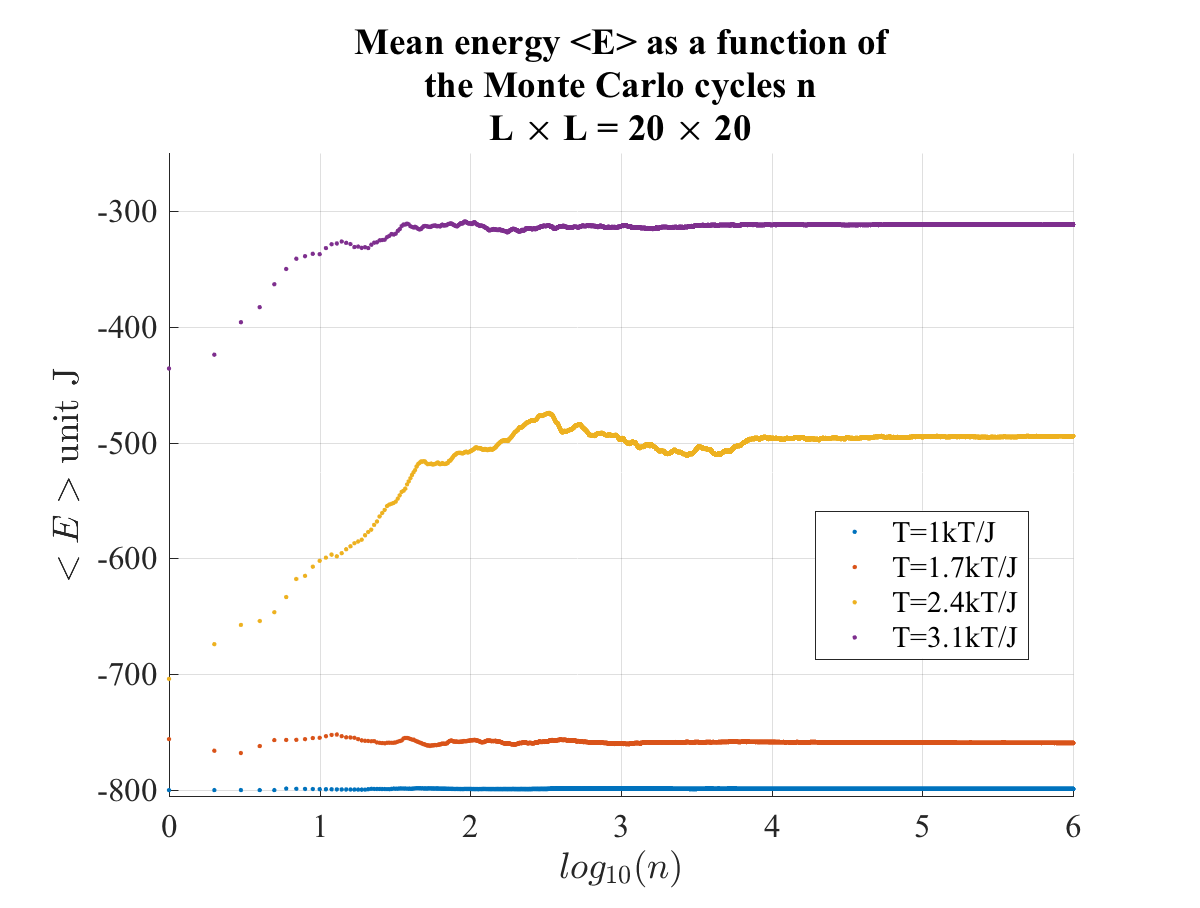
\includegraphics[width=.5\linewidth]{e20x20.eps}\label{e20x20}}
%     \subfloat[]{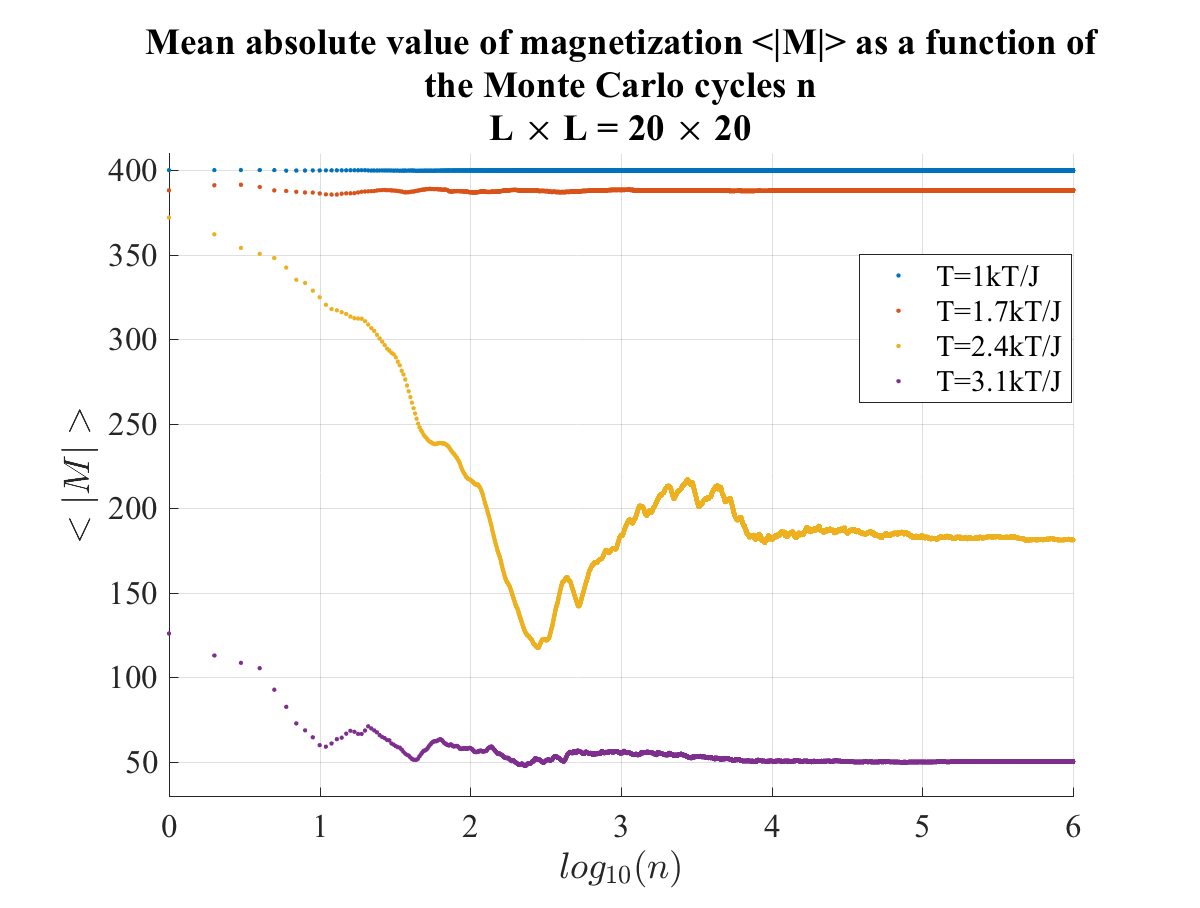
\includegraphics[width=.5\linewidth]{absm20x20.eps}\label{absm20x20.eps}}
%\caption{In Figure (a) and (b) are shown respectively mean energy and mean absolute value of magnetization as a function of Monte Carlo cycles $n$ for different temperatures and lattice dimension $L=20$. At temperature $2.4 kT/J$ both the quantities take more time to reach a steady state.}
%\end{figure}

\section{Conclusion}
%State your main findings and interpretations
%Try as far as possible to present perspectives for future work
%Try to discuss the pros and cons of the methods and possible improvements




%\section{Acknowledgments}
% \section{\label{sec:level1}First-level heading}

% This sample document demonstrates proper use of REV\TeX~4.1 (and
% \LaTeXe) in mansucripts prepared for submission to APS
% journals. Further information can be found in the REV\TeX~4.1
% documentation included in the distribution or available at
% \url{http://authors.aps.org/revtex4/}.

% When commands are referred to in this example file, they are always
% shown with their required arguments, using normal \TeX{} format. In
% this format, \verb+#1+, \verb+#2+, etc. stand for required
% author-supplied arguments to commands. For example, in
% \verb+\section{#1}+ the \verb+#1+ stands for the title text of the
% author's section heading, and in \verb+\title{#1}+ the \verb+#1+
% stands for the title text of the paper.

% Line breaks in section headings at all levels can be introduced using
% \textbackslash\textbackslash. A blank input line tells \TeX\ that the
% paragraph has ended. Note that top-level section headings are
% automatically uppercased. If a specific letter or word should appear in
% lowercase instead, you must escape it using \verb+\lowercase{#1}+ as
% in the word ``via'' above.

% \subsection{\label{sec:level2}Second-level heading: Formatting}

% This file may be formatted in either the \texttt{preprint} or
% \texttt{reprint} style. \texttt{reprint} format mimics final journal output. 
% Either format may be used for submission purposes. \texttt{letter} sized paper should
% be used when submitting to APS journals.

% \subsubsection{Wide text (A level-3 head)}
% The \texttt{widetext} environment will make the text the width of the
% full page, as on page~\pageref{eq:wideeq}. (Note the use the
% \verb+\pageref{#1}+ command to refer to the page number.) 
% \paragraph{Note (Fourth-level head is run in)}
% The width-changing commands only take effect in two-column formatting. 
% There is no effect if text is in a single column.

% \subsection{\label{sec:citeref}Citations and References}
% A citation in text uses the command \verb+\cite{#1}+ or
% \verb+\onlinecite{#1}+ and refers to an entry in the bibliography. 
% An entry in the bibliography is a reference to another document.

% \subsubsection{Citations}
% Because REV\TeX\ uses the \verb+natbib+ package of Patrick Daly, 
% the entire repertoire of commands in that package are available for your document;
% see the \verb+natbib+ documentation for further details. Please note that
% REV\TeX\ requires version 8.31a or later of \verb+natbib+.

% \paragraph{Syntax}
% The argument of \verb+\cite+ may be a single \emph{key}, 
% or may consist of a comma-separated list of keys.
% The citation \emph{key} may contain 
% letters, numbers, the dash (-) character, or the period (.) character. 
% New with natbib 8.3 is an extension to the syntax that allows for 
% a star (*) form and two optional arguments on the citation key itself.
% The syntax of the \verb+\cite+ command is thus (informally stated)
% \begin{quotation}\flushleft\leftskip1em
% \verb+\cite+ \verb+{+ \emph{key} \verb+}+, or\\
% \verb+\cite+ \verb+{+ \emph{optarg+key} \verb+}+, or\\
% \verb+\cite+ \verb+{+ \emph{optarg+key} \verb+,+ \emph{optarg+key}\ldots \verb+}+,
% \end{quotation}\noindent
% where \emph{optarg+key} signifies 
% \begin{quotation}\flushleft\leftskip1em
% \emph{key}, or\\
% \texttt{*}\emph{key}, or\\
% \texttt{[}\emph{pre}\texttt{]}\emph{key}, or\\
% \texttt{[}\emph{pre}\texttt{]}\texttt{[}\emph{post}\texttt{]}\emph{key}, or even\\
% \texttt{*}\texttt{[}\emph{pre}\texttt{]}\texttt{[}\emph{post}\texttt{]}\emph{key}.
% \end{quotation}\noindent
% where \emph{pre} and \emph{post} is whatever text you wish to place 
% at the beginning and end, respectively, of the bibliographic reference
% (see Ref.~[\onlinecite{witten2001}] and the two under Ref.~[\onlinecite{feyn54}]).
% (Keep in mind that no automatic space or punctuation is applied.)
% It is highly recommended that you put the entire \emph{pre} or \emph{post} portion 
% within its own set of braces, for example: 
% \verb+\cite+ \verb+{+ \texttt{[} \verb+{+\emph{text}\verb+}+\texttt{]}\emph{key}\verb+}+.
% The extra set of braces will keep \LaTeX\ out of trouble if your \emph{text} contains the comma (,) character.

% The star (*) modifier to the \emph{key} signifies that the reference is to be 
% merged with the previous reference into a single bibliographic entry, 
% a common idiom in APS and AIP articles (see below, Ref.~[\onlinecite{epr}]). 
% When references are merged in this way, they are separated by a semicolon instead of 
% the period (full stop) that would otherwise appear.

% \paragraph{Eliding repeated information}
% When a reference is merged, some of its fields may be elided: for example, 
% when the author matches that of the previous reference, it is omitted. 
% If both author and journal match, both are omitted.
% If the journal matches, but the author does not, the journal is replaced by \emph{ibid.},
% as exemplified by Ref.~[\onlinecite{epr}]. 
% These rules embody common editorial practice in APS and AIP journals and will only
% be in effect if the markup features of the APS and AIP Bib\TeX\ styles is employed.

% \paragraph{The options of the cite command itself}
% Please note that optional arguments to the \emph{key} change the reference in the bibliography, 
% not the citation in the body of the document. 
% For the latter, use the optional arguments of the \verb+\cite+ command itself:
% \verb+\cite+ \texttt{*}\allowbreak
% \texttt{[}\emph{pre-cite}\texttt{]}\allowbreak
% \texttt{[}\emph{post-cite}\texttt{]}\allowbreak
% \verb+{+\emph{key-list}\verb+}+.

\section{Bibliography}
\begin{itemize}

\item M. H. Jensen, \textit{Computational physics - Lecture notes Fall 2015}, University of Oslo - Department of Physics, 2015. 

\end{itemize}

\end{document}
